\chapter{Implementation}
\label{chap:implementation}

\section{Architecture}

\begin{figure}
    \centering
    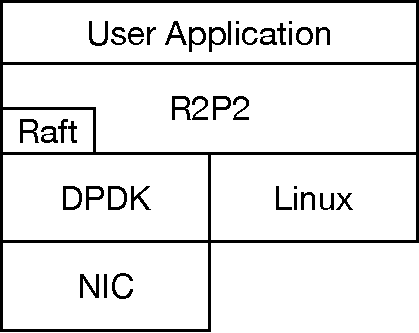
\includegraphics[width=0.4\textwidth]{system_layers}
    \caption{View of the different layers in the system architecture.
    \label{fig:architecture}
    }
\end{figure}

The global architecture of our system can be seen on Figure~\ref{fig:architecture}.
At the top sits the application logic, which can be any general networked application: HTTP server, database, cache, \etc
The implementation presented in this report can accomodate any of those.

The application layer uses services provided by the \gls{r2p2} library.
The main role of this library is to assemble complete \gls{rpc} messages from \gls{udp} datagrams.
It also handles the logic of replying to a given request, as well as some acknowledgements required for load balancing.
This layer also provides networked I/O to the Raft implementation.

The \gls{r2p2} layer will in turn make calls into DPDK and Linux for various functionalities.
We must emphasize that all the ``hot path'' operations are done through DPDK, as calling into Linux is too slow for our purposes.
Not shown here is also a small \gls{udp}/IP stack, with support for auxiliary features like the \gls{arp}.


\section{Implementation language}

As the reference implementation of \gls{r2p2} was written in C, we wanted to use a language that could be easily integrated with the existing codebase.
We decided to use C++ for the gain in expressiveness compared to pure C.
In particular, templates allow code to be easily written in a generic fashion.
Move semantics are also available in this language since C++11, and allow us to avoid a lot of packet copying while simplifying memory management.
While not as useful as Rust's, mostly due to the lack of safety guarantees, they still form a very useful tool to reduce packet copying while simplifying memory management.

\section{Message Routing}
\label{sec:message_routing}

In Raft, only the leader can process new client requests.
This keeps the protocol simpler by only having data flowing from the leader to the followers.
On the other hand, it means that we must also have a way to direct client queries to the leader.

In the original Raft paper\cite{raft}, the followers will redirect clients to the leader if contacted directly.
However, this is not optimal from a tail latency perspective: a client that picks a follower as a destination will see an additional \gls{rtt} to its request.

Fortunately, \gls{r2p2} was implemented with load balancing semantics in mind.
We can therefore extend the \gls{r2p2} load balancer to always propagate replicated requests to the current leader.
While this haven't been done yet, it could be implementing by having the load balancer listening to Raft heartbeat messages (Figure~\ref{fig:r2p2_raft_routing}).

For our benchmarking we manually pointed the benchmark client to the elected leader.

\begin{figure}
    \centering
    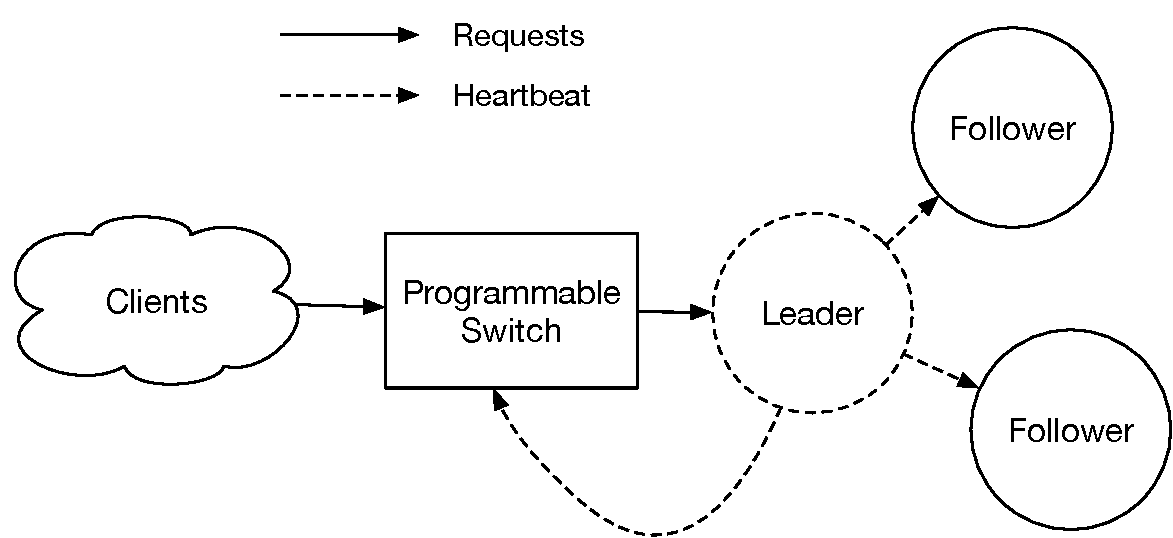
\includegraphics[width=0.8\textwidth]{r2p2_raft_routing}
    \caption{Message routing with R2P2 and Raft.
        The programmable switch listens to Raft leader heartbeats and forwards requests to the leader with the highest term.
    \label{fig:r2p2_raft_routing}
    }
\end{figure}

\section{Log}

At the end, Raft can only replicate a log, and ensure that all the nodes will eventually have all entries, in the same order.
We must provide an adequate definition of the log entries for our needs.
Since we are using Raft to replicate \gls{rpc} requests, the log entries will contain a \gls{r2p2} request: A source address and port, a request ID, and the request data.

To keep things simple and low latency, our log implementation stores its data in RAM only.
The requests are kept in a circular buffers, so that the oldest entry gets replaced by the newest one.
The data is stored into the circular buffer without copying; when an entry is overwritten, its data is given back to the network stack.

\section{Worker threads}

During evaluation of the original design, we discovered that executing the workloads in the main thread created a lot of queueing (Section~\ref{sec:latency_throughput}).
Because of this, we decided to move the processing of the workloads off the main networking thread and into auxiliary workers.
Data between the two is passed through queues.

However, simply using threadsafe queues would not have been enough.
The overhead from mutexes can be quite important, reducing total throughput.
The chosen approach is to use lockless queues, in which one reader thread can access the tail pointer, and one writer thread can access the head pointer.
Since the pointers are not written by both threads and can only move in one direction (head cannot move back), it is safe to share the data structure without synchronization.
We used an existing high performance implementation\cite{fast_queue}, as writing such data structures is error-prone and out of the scope of this thesis.

One downside of the current approach is that requests in the leader node are still executed by the main/network thread.
This was done to avoid copying reponse data from one thread to another.
However, it could cause some issues when a node transitions from follower to leader, if the application code is not thread safe.

\section{DPDK backend}

In order to provide the best performance, \gls{r2p2} implements kernel bypass technologies.
In this mode, the application talks directly to a dedicated \gls{nic}, embedding the driver in the library code.

For the implementation we opted to use Intel's DPDK framework.
Several other kernel bypass framework exist such as netmap\cite{netmap}, or Ixy\cite{ixy}.
However they do not appear to have the same industrial traction as DPDK, neither are they cross platform; DPDK can run on Linux and FreeBSD on both Intel and ARM processors.

\section{Userland backend}

While kernel bypass offers the best performance, it is not always possible to use it (\ie when using a \gls{nic} is shared between applications).
Our current implementation can therefore either be compiled to use DPDK (and a custom UDP/IP stack) or to use the normal kernel networking facilities.
In this second case, only \gls{r2p2} is implemented in the application; the rest runs in-kernel.

To achieve high performance and stay close to DPDK's event based model, we use asynchronous I/O facilities.
Our first implementation used Linux's \texttt{epoll} directly, making it non-portable.
We rewrote it to use libuv instead, which abstracts the different asynchronous I/O mechanisms on Linux, BSD and Windows.

This means that the current implementation can run as a normal networked component on all major platforms.
This allows for a much easier development experience than running DPDK directly, and can even be used in production with good performance.

\section{Timers}

The Raft algorithm relies a lot on timers to detect leader absence and organize elections.
In order to implement this, we simply use the functions provided by both Intel's DPDK and libuv.
The port layer must only periodically call a function (\texttt{raft\_tick}).
This call is then used to process timeouts in various parts of the Raft implementation.

\section{Modification to client libraries}

On the client side, the code requires very little modifications to work with replicated request.
One should just add the new routing policy definition.
Nothing else is changed, and the client will still send and receive only one request response pair.


\section{Implementation complexity}

Our code can be divided in two big parts.
The first one is the Raft logic implementation, which does not do any I/O, timer management, \etc
It is about a thousand line of C++ code, which uses a lot templates and the standard library collections.
In addition comes about 1500 lines of unit testing, very useful to check the soundness of our Raft code.

The second part is the part specific to \gls{r2p2}, which implements custom log entries for \gls{r2p2} requests.
This amounts to 250 lines of C++.

Finally we have a few changes to the core code in C, but they stay quite small.
It mostly consists of routing requests tagged with \texttt{REPLICATED\_ROUTE} to the Raft code.
